\documentclass[11pt,letterpaper]{article}
\usepackage{geometry}
\usepackage[utf8]{inputenc}
\usepackage{natbib}
\usepackage{lscape}
\usepackage{amsmath}
\usepackage{amsfonts}
\usepackage{amsthm}
\usepackage{amssymb}
\usepackage{mathtools}
\usepackage{graphicx}
\usepackage{multicol}
\usepackage{subfig}
\usepackage{float}
\usepackage{algpseudocode}
\usepackage{fancyhdr}
\usepackage{enumitem}
\usepackage[hidelinks]{hyperref}

\geometry{verbose,letterpaper,tmargin=3cm,bmargin=3cm,lmargin=2.5cm,rmargin=2.5cm}

% Tables
\usepackage{multirow}
\usepackage[table]{xcolor}

% Avoid to split words at the end of each line
\usepackage[none]{hyphenat}

\newcommand{\NN}{{\mathbb{N}}}
\newcommand{\LL}{{\mathbb{L}}}
\newcommand{\ZZ}{{\mathbb{Z}}}
\newcommand{\QQ}{{\mathbb{Q}}}
\newcommand{\RR}{{\mathbb{R}}}
\newcommand{\WW}{{\mathbb{W}}}
\newcommand{\CC}{{\mathbb{C}}}
\newcommand{\HH}{{\mathbb{H}}}
\newcommand{\FF}{{\mathbb{F}}}
\newcommand{\PP}{{\mathbb{P}}}
\newcommand{\U}{{\mathcal{U}}}
\newcommand{\A}{{\mathcal{A}}}
\newcommand{\M}{{\mathcal{M}}}
\newcommand{\X}{{\mathcal{X}}}
\newcommand{\F}{{\mathcal{F}}}
\newcommand{\el}{{\mathcal{L}}}
\newcommand{\R}{{\mathcal{R}}}

\let\originalleft\left
\let\originalright\right
\renewcommand{\left}{\mathopen{}\mathclose\bgroup\originalleft}
\renewcommand{\right}{\aftergroup\egroup\originalright}

\newcommand{\norm}[1]{\left\lVert#1\right\rVert}

\theoremstyle{definition}
\newtheorem{definition}{Definition}[section]
\newtheorem{theorem}{Theorem}[section]
\newtheorem{corolary}{Corolary}[section]

\author{David Plazas$^\dag$ \\\vspace{0.3cm}\small{dplazas@eafit.edu.co}\\
$^\dag$Mathematical Engineering, Universidad EAFIT}



\title{Final Report: Analysis II}

\sloppy

\begin{document}

\maketitle
\section{Modes of Convergence}
This section is based on Chapter 4 from \cite{myriam2002introduccion}. The definitions and theorems will be stated, and the theorems between modes of convergence will be finally represented with a chart.

\subsection{$\LL^p_m(\Omega)$ spaces}
\begin{definition}
Let $(\Omega,\, \mathcal{A},\, \mu)$ be a measure space. $\el^p_m(\Omega)$ is the set of all measurable functions $g:\Omega\rightarrow\RR^m$ that satisfy 
\begin{equation}
    \mathcal{N}_p(g):=\left(\int_\Omega\left|g\right|^pd\mu\right)^{1/p}<\infty, \ 1\leq p<\infty
\end{equation}
\end{definition}

\begin{theorem}[H\"older's Inequality]
Let $(\Omega,\, \mathcal{A},\, \mu)$ be a measure space. Let $p\in\RR$, with $1<p<\infty$ and let $q$ be such that $\frac{1}{p} + \frac{1}{q}=1$. Then for all measurable functions $f$ and $g$, defined over $\Omega$ we have
\begin{equation}
    \int_\Omega\left|fg\right|d\mu \leq \left(\int_\Omega\left|f\right|^pd\mu\right)^{1/p}\left(\int_\Omega\left|g\right|^qd\mu\right)^{1/q}
\end{equation}
which directly implies that if $f(\cdot)\in\el^p_m(\Omega)$ and $g(\cdot)\in\el_m^q(\Omega)$, then $(fg)(\cdot)\in\el^1_m(\Omega)$.
\end{theorem}

\begin{theorem}[Minkowski's Inequality]
Let $(\Omega,\, \mathcal{A},\, \mu)$ be a measure space. Let $f(\cdot)\in\el^p_m(\Omega)$ and $g\in\el^p_m(\Omega)$ with $1\leq p < \infty$, such that their sum $f+g$ is defined a.e. on $\Omega$. Then
\begin{equation}
    \left(\int_\Omega\left|f+g\right|^pd\mu\right)^{1/p} \leq \left(\int_\Omega\left|f\right|^pd\mu\right)^{1/p} + \left(\int_\Omega\left|g\right|^pd\mu\right)^{1/p}
\end{equation}
\end{theorem}
\begin{theorem}
Let $(\Omega,\, \mathcal{A},\, \mu)$ be a measure space. Let $f(\cdot)\in\el^p_m(\Omega)$ and $g\in\el^p_m(\Omega)$ with $1\leq p < \infty$. Let $c\in\RR$. Then:
\begin{multicols}{2}
\begin{enumerate}
    \item $cf(\cdot)\in \el^p_m(\Omega)$
    \item $(f+g)(\cdot)\in \el^p_m(\Omega)$
    \columnbreak
    \item $\sup\{f,g\}(\cdot)\in \el^p_m(\Omega)$
    \item $\inf\{f,g\}(\cdot)\in \el^p_m(\Omega)$
\end{enumerate}
\end{multicols}
\end{theorem}

It can be proved tha the function $\mathcal{N}_p(\cdot)$ is a seminorm (or pseudonorm) in $\el^p_m(\Omega)$, since it allows zero values for nonzero elements of $\el^p_m(\Omega)$. This is due to the presence of functions, for example, $f(\omega)=0$ a.e. on $\Omega$, since the $\mu$-integral of such functions is 0 but clearly the functions are not completely null. The following definition addresses this issue and defines the $\LL_m^p(\Omega)$ spaces.


\begin{definition}
Let $(\Omega,\,\A,\,\mu)$ be a measure space. Let $1\leq p<\infty$. Define the equivalence relation in $\el^p_m(\Omega)$ as: $f\sim g \iff f=g$ a.e. on $\Omega$. The normed vector space $\LL_m^p(\Omega)$ is the defined as the set of equivalence classes of functions in $\el^p_m(\Omega)$. If $f(\cdot)\in\el^p_m(\Omega)$, let us denote $[f(\cdot)]$ as the equivalence class of $f(\cdot)$. The norm in $\LL_m^p(\Omega)$ for a function $f(\cdot)$ is $\norm{[f(\cdot)]}_p:=\mathcal{N}_p(f)$.
\end{definition}

\subsection{Modes of Convergence}
The section assumes a measure space $(\Omega,\,\A,\,\mu)$.
\begin{definition}
A sequence $\{f_n(\cdot)\}_{n\in\NN}$ of functions in $\LL_m^p(\Omega)$ converges in $p$-mean to a function $f(\cdot)\in \LL_m^p(\Omega)$ if
\begin{equation}
    \lim_{n\rightarrow\infty}\int_\Omega\left|f_n-f\right|^pd\mu = 0,
\end{equation}
and it is written as $f_n\xrightarrow[n\rightarrow\infty]{\LL_m^p(\Omega)}f$.
\end{definition}
\begin{theorem}
If $f_n\xrightarrow[n\rightarrow\infty]{\LL_m^p(\Omega)}f$ and $f_n\xrightarrow[n\rightarrow\infty]{\LL_m^p(\Omega)}g$ then $f=g$ a.e. on $\Omega$.
\end{theorem}

\begin{definition}
A sequence $\{f_n(\cdot)\}_{n\in\NN}$ of measurable functions converges almost everywhere (a.e. convergent) to $f(\cdot)$ if 
\begin{equation}
    \lim_{n\rightarrow\infty}f_n = f \ \text{a.e. on } \Omega
\end{equation}
and it is written as $f_n\xrightarrow[n\rightarrow\infty]{\text{a.e.}}f$.
\end{definition}

\begin{theorem}[Lebesgue's Dominated Convergence]
Let $\{f_n(\cdot)\}_{n\in\NN}$ be a sequence a.e. convergent in $\LL_m^p(\Omega)$. Assuming that $\exists g:\Omega\rightarrow\RR^m_+$ such that $g(\cdot)\in\LL_m^p(\Omega)$ and $\left|f_n\right|\leq g$, $\forall n\in\NN$, then
\begin{enumerate}
    \item $\exists f:\Omega\rightarrow\RR^m$ measurable such that $f_n\xrightarrow[n\rightarrow\infty]{\text{a.e.}}f$.
    \item for each measurable function $f:\Omega\rightarrow\RR^m$ that satisfies $f_n\xrightarrow[n\rightarrow\infty]{\text{a.e.}}f$, then $f(\cdot)\in\LL_m^p(\Omega)$ and $f_n\xrightarrow[n\rightarrow\infty]{\LL_m^p(\Omega)}f$.
\end{enumerate}
\end{theorem}

\begin{definition}
A sequence $\{f_n(\cdot)\}_{n\in\NN}$ of functions in $\LL_m^p(\Omega)$ is a Cauchy sequence in $\LL_m^p(\Omega)$ if $\forall \epsilon>0, \ \exists N\in\NN$ such that $\norm{[f_n(\cdot)-f_m(\cdot)]}_p\leq\epsilon$, $\forall n,m\geq N$.
\end{definition}
\begin{theorem}
Let $\{f_n(\cdot)\}_{n\in\NN}$ be a sequence in $\LL_m^p(\Omega)$. Let $f(\cdot)\in\LL_m^p(\Omega)$. Then, $f_n\xrightarrow[n\rightarrow\infty]{\LL_m^p(\Omega)}f$ if and only if $\{f_n(\cdot)\}_{n\in\NN}$ is a Cauchy sequence in $\LL_m^p(\Omega)$. Moreover, there exists a subsequence that converges a.e. on $\Omega$ to $f(\cdot)$, for $1\leq p<\infty$.
\end{theorem}

\begin{theorem}
If $\{f_n(\cdot)\}_{n\in\NN}$ converges in $p$-mean to $f(\cdot)\in\LL_m^p(\Omega)$, with $1\leq p<\infty$, then $\norm{[f_n(\cdot)]}_p\rightarrow\norm{[f(\cdot)]}_p$ (let us call this ``convergence of norms'').
\end{theorem}

\begin{theorem}
Let $\{f_n(\cdot)\}_{n\in\NN}$ be a sequence in $\LL_m^p(\Omega)$, $f(\cdot)\in\LL_m^p(\Omega)$, $1\leq p<\infty$ and $f_n\xrightarrow[n\rightarrow\infty]{\text{a.e.}}f$. If $\norm{[f_n(\cdot)]}_p\rightarrow\norm{[f(\cdot)]}_p$, then $f_n\xrightarrow[n\rightarrow\infty]{\LL_m^p(\Omega)}f$.
\end{theorem}

\begin{definition}
The sequence $\{f_n(\cdot)\}_{n\in\NN}$ of functions $f_i:\Omega\rightarrow\RR, \ \forall i\in\NN$ converges in measure to a measurable function $f(\cdot)$ if
\begin{equation}
\lim_{n\rightarrow\infty}\mu\left(\left\{\omega\in\Omega: \left|f_n(\omega)-f(\omega)\right|\geq\alpha\right\}\cap A\right)=0
\end{equation}
for $\alpha>0$ and $\forall A\in\A$ such that $\mu(A)<\infty$. It is written as $f_n\xrightarrow[n\rightarrow\infty]{\mu}f$. Furthermore, the sequence $\{f_n(\cdot)\}_{n\in\NN}$ is said to be Cauchy on measure if 
\begin{equation}
\lim_{n,m\rightarrow\infty}\mu\left(\left\{\omega\in\Omega: \left|f_n(\omega)-f_m(\omega)\right|\geq\alpha\right\}\cap A\right)=0
\end{equation}
for $\alpha>0$ and $\forall A\in\A$ such that $\mu(A)<\infty$.
\end{definition}

\begin{definition}
The sequence $\{f_n(\cdot)\}_{n\in\NN}$ of functions $f_i:\Omega\rightarrow\RR, \ \forall i\in\NN$ converges uniformly to $f(\cdot)$ if, given $\epsilon>0$, $\exists N\in\NN$ such that $\forall n\geq N$,
\begin{equation}
    \left|f_n(\omega)-f(\omega)\right|<\epsilon,\ \forall\omega\in\Omega
\end{equation}
and it is written as $f_n\rightrightarrows f$.
\end{definition}
\begin{theorem}
If a sequence $\{f_n(\cdot)\}_{n\in\NN}$ converges uniformly to $f(\cdot)$ then it converges in measure to $f(\cdot)$.
\end{theorem}

\begin{theorem}
The convergence in $p$-mean in $\LL_m^p(\Omega)$ implies the convergence in measure.
\end{theorem}

\begin{theorem}
If a sequence $\{f_n(\cdot)\}_{n\in\NN}$ of functions $f_i:\Omega\rightarrow\RR, \ \forall i\in\NN$ is Cauchy on measure, then there exists a subsequence that converges on measure and a.e. on $\Omega$ to a measurable function $f:\Omega\rightarrow\RR$.
\end{theorem}

\begin{theorem}
If a sequence $\{f_n(\cdot)\}_{n\in\NN}$ of functions $f_i:\Omega\rightarrow\RR, \ \forall i\in\NN$ is Cauchy on measure, then $\exists f:\Omega\rightarrow\RR$ such that $f_n\xrightarrow[n\rightarrow\infty]{\mu}f$ and it is determined a.e. on $\Omega$.
\end{theorem}

\begin{theorem}
Let $\{X_n\}_{n\in\NN}$ be sequence of random variables defined on a probability space $(\Omega,\A,P)$. If $X_n\xrightarrow[n\rightarrow\infty]{\text{a.e.}}X$, then $X_n\xrightarrow[n\rightarrow\infty]{P}X$.
\end{theorem}

\begin{theorem}
Let $\{f_n(\cdot)\}_{n\in\NN}$ be sequence of functions in $\LL_m^p(\Omega)$ that converges in measure to $f(\cdot)$ and let $g(\cdot)\in\LL_m^p(\Omega)$ such that $\forall n\in\NN,\ |f_n(\omega)|\leq g(\omega)$ a.e. on $\Omega$. Then, $f(\cdot)\in\LL_m^p(\Omega)$ and $f_n\xrightarrow[n\rightarrow\infty]{\LL_m^p(\Omega)}f$.
\end{theorem}

\begin{definition}
A sequence $\{f_n(\cdot)\}_{n\in\NN}$ of measurable functions $f_i:\Omega\rightarrow\RR, \ \forall i\in\NN$, is said to be almost uniformly convergent to a measurable function $f(\cdot)$ if for each $\epsilon>0$, $\exists E_\epsilon\in\A$ with $\mu(E_\epsilon)<\epsilon$ and such that $\{f_n(\cdot)\}_{n\in\NN}$ converges uniformly to $f(\cdot)$ in $E_\epsilon^c$.
\end{definition}

\begin{theorem}
Let $\{f_n(\cdot)\}_{n\in\NN}$ be sequence of functions $f_i:\Omega\rightarrow\RR, \ \forall i\in\NN$ that converges almost uniformly to a measurable function $f:\Omega\rightarrow \RR$. Then $f_n\xrightarrow[n\rightarrow\infty]{\mu}f$ and $f_n\xrightarrow[n\rightarrow\infty]{\text{a.e.}}f$.
\end{theorem}

\begin{theorem}
Let $\{f_n(\cdot)\}_{n\in\NN}$ be a sequence that converges in measure to $f(\cdot)$, then there exists a subsequence that converges almost uniformly (particularly, a.e. convergent) to the same function $f(\cdot)$. 
\end{theorem}

\begin{theorem}
Let $\{f_n(\cdot)\}_{n\in\NN}$ be a sequence of functions in $\LL_m^p(\Omega)$, with $1\leq p<\infty$. The following are necessary and sufficient conditions for the $p$-mean convergence to $f(\cdot)$:
\begin{enumerate}
    \item $\{f_n(\cdot)\}_{n\in\NN}$ converges to $f(\cdot)$ in measure.
    \item $\forall \epsilon>0,\,\exists E_\epsilon\in\A$ with $\mu\left(E_\epsilon\right)<\infty$ and such that if $A\in\A$ and $A\cap E_\epsilon=\phi$, then
    \begin{equation}
        \int_A\left|f_n\right|^pd\mu<\epsilon^p, \ \forall n\in\NN.
    \end{equation}
    \item $\forall \epsilon>0,\,\exists\delta>0$ such that if $E\in\A$ and $\mu(E)<\delta$, then
    \begin{equation}
        \int_E\left|f_n\right|^pd\mu<\epsilon^p, \ \forall n\in\NN.
    \end{equation}
\end{enumerate}
\end{theorem}

\begin{theorem}
Let $(\Omega,\A, \mu)$ be a finite measure space. Let $\{f_n(\cdot)\}_{n\in\NN}$ be a sequence of measurable functions $f_i:\Omega\rightarrow\RR, \ \forall i\in\NN$, that converges a.e. to a measurable function $f:\Omega\rightarrow\RR$. Then, $\{f_n(\cdot)\}_{n\in\NN}$ converges almost uniformly to $f(\cdot)$.
\end{theorem}

Let us present a chart of that summarizes the implications between the modes of convergence in Figure \ref{fig:chart}. The legend of types of implications is within the figure, each mode of convergence has a number above representing the definition number within this document, and the numbers in the arrows represent the theorem that states the relationship.

\begin{figure}[ht]
    \centering
    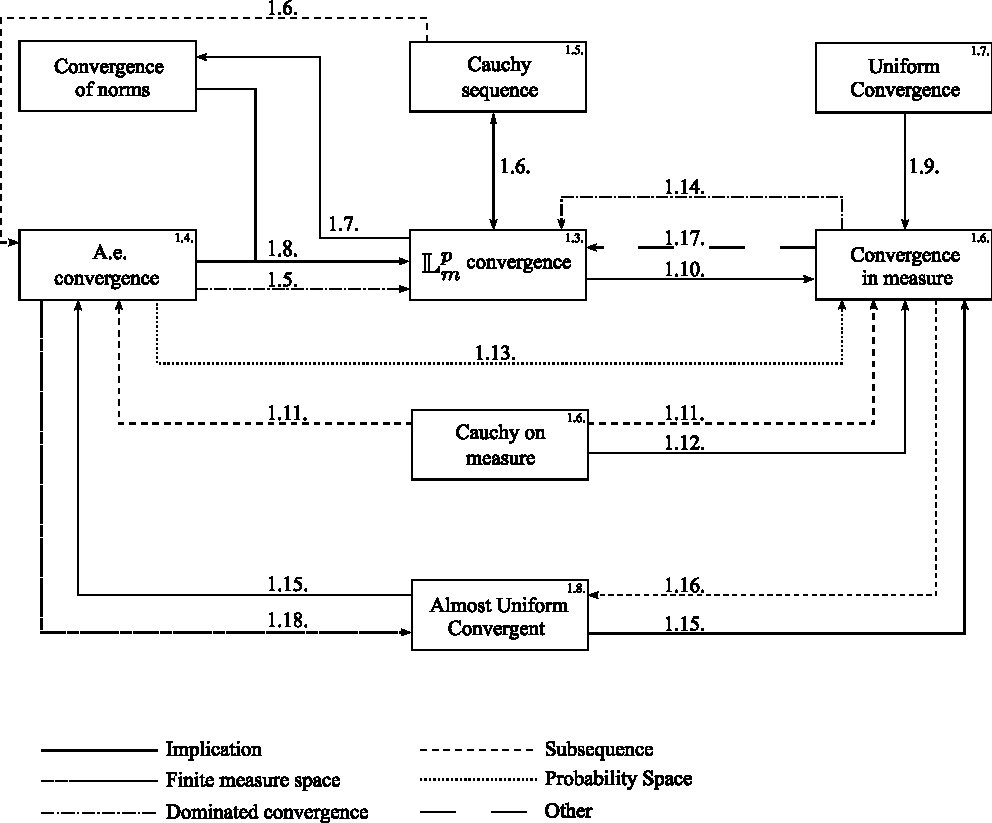
\includegraphics[width=\textwidth]{figs/diag_mc.pdf}
    \caption{Implications between modes of convergence.}
    \label{fig:chart}
\end{figure}


%%%%%%%%%%%%%%%%%%%%%%%%%%%%%%%%%%%%%
\section{Vadim Lectures}
This section briefly describes some necessary concepts for the further development of the tasks assigned and some concepts mentioned during prof. Vadim lectures. Most ideas are extracted from \cite{azhmyakov2011approximability}.

\begin{definition}
A control system with the explicit form
\begin{equation}\label{eq:ca_sys}
    \begin{split}
    &\dot{x}(t)=a\left(t,x(t)\right) + b\left(t,x(t)\right)u(t), \ \text{a.e. on } [0, t_f],\\
    &x(0)=x_0\in\RR^n
    \end{split}
\end{equation}
is called a control-affine (CA) system.
\end{definition}

\begin{definition}
A function $f(t,x)$, with type $f:(0,t_f)\times\R\rightarrow\RR^n$, is called uniformly Lipschitz continuous in $x$ if, for almost all t, $\exists K\in \RR$ such that $\forall x_1,x_2\in\R_+$
\begin{equation}
    \norm{f(t,x_1)-f(t,x_2)}\leq K\norm{x_1-x_2}.
\end{equation}
\end{definition}

\begin{definition}
Let $(Y, d)$ a metric space. A set of functions, $\F:=\{f_i:(0,t_f)\times\mathcal{R}\rightarrow Y,\,i\in I\}$ is uniformly bounded if $\exists y\in Y$ such that $d\left(f_i(t,x),y\right)\leq M$, $\forall i\in I$ and $\forall t,x\in(0,t_f)\times\R$, with $M\in\RR_+$.
\end{definition}

The following assumptions are natural when dealing with CA systems: 
\begin{enumerate}
    \item[i)] The control is a function $u:[0,t_f]\rightarrow\RR^m$.
    \item[ii)] The functions $a:[0,t_f]\times\R\rightarrow\RR^n$ and $b:[0,t_f]\times\R\rightarrow\RR^{n\times m}$ are uniformly bounded on an open set $(0,t_f)\times\R\subseteq\RR^{n+1}$.
    \item[iii)] The functions $a(t,x)$ and $b(t,x)$ are measurable w.r. to $t\in(0,t_f)$.
    \item[iv)] The functions $a(t,x)$ and $b(t,x)$ uniformly Lipschitz continuous w.r. to $x$ (with a common constant for almost all t).
\end{enumerate}
These assumptions imply that the right-hand side of the control system (\ref{eq:ca_sys}) is a Carathéodory function, which allows the CA system to an absolutely continuous solution $x^u(\cdot)$, for every $u(\cdot)\in\LL^1_m(0,t_f)$. Carathéodory's existence theorem is an extension of Peano's classic existence theorem for initial value problems involving ordinary differential equations.

\begin{definition}
A function $f:[a,b]\rightarrow\RR$ is absolutely continuous if $f'(\cdot)\in\LL_1^1([a,b])$ and 
\begin{equation}
    f(t)-f(a)=\int_a^xf'(t)dt,\ \forall t\in[a,b].
\end{equation}
\end{definition}
This fact makes it possible to define a set $\mathrm{AC}[a,b]$ of absolutely continuous functions in $[a,b]$, which is a subset of the space of continuous functions in $[a,b]$, denoted by $\CC[a,b]$.
\begin{definition}
Let $0<p<\infty$. We define the dual of $\LL_m^p(0,t_f)$, sometimes denoted $\left(\LL_m^p(0,t_f)\right)^*$, as the space $\LL_m^{p'}(0,t_f)$, where $p'$ satisfies $\frac{1}{p} + \frac{1}{p'}=1$. If $p=1$, the dual of $\LL_m^1(0,t_f)$ is $\LL^\infty_m(0,t_f)$.
\end{definition}
Some useful properties of the dual in Lebesgue spaces are: i) $\left(\LL_m^{p'}(0,t_f)\right)^*=\LL^p_m(0,t_f)$, ii) $\LL^2_m(0,t_f)$ is a Hilbert space with scalar product, iii) $\LL^1_m(0,t_f)\subset\left(\LL_m^\infty(0,t_f)\right)^*$.

\begin{definition}
A sequence $\{u^{(k)(\cdot)}\}_{k\in\NN}$ of functions in $\LL^p_m(0,t_f)$ is said to converge weakly to a function $u(\cdot)\in\LL^p_m(0,t_f)$ if
\begin{equation}
    \lim_{k\rightarrow\infty}\left\langle u^{(k)}(\cdot),v(\cdot)\right\rangle_{p,p'}=\langle u(\cdot),v(\cdot)\rangle_{p,p'},\quad\forall v(\cdot)\in\LL_m^{p'}(0,t_f),
\end{equation}
where $\langle\cdot,\cdot\rangle$ is the fundamental linear form associated with both original and dual spaces. This means the application if a linear functional from one space to an element of the other. For the applications of Vadim's theorems, we consider the specific case $p=1$ and $p'=\infty$, where these brackets translate into
\begin{equation}
    \langle u(\cdot),v(\cdot)\rangle_{1,\infty}=\int_{(0,t_f)}u(t)v(t)dt,
\end{equation}
where clearly $u(\cdot)\in\LL_m^1(0,t_f)$ and $v(\cdot)\in\LL^\infty_m(0,t_f)$.
\end{definition}

\begin{theorem}[Azhmyakov's Theorem 1]\label{th:1}
Let $\X$ be a separable Banach space and let $(\Omega,\A,P)$ be a probability space. Let $C\subset\X$ be closed and convex. If $h:\Omega\rightarrow C$ is a measurable function, then 
\begin{equation}
\int_\Omega hdP\in C.
\end{equation}
\end{theorem}

\begin{theorem}[Azhmyakov's Theorem 2]\label{th:2}
Consider a CA system like (\ref{eq:ca_sys}), an associated sequence $\{u^{(k)}(\cdot)\}_{k\in\NN}$ of control functions in $\LL_m^1(0,t_f)$ such that $\{u^{(k)}(\cdot)\}_{k\in\NN}$ converges weakly to an element $u(\cdot)\in\LL_m^1(0,t_f)$, and a sequence of vectors $\{x_0^{(k)}\}_{k\in\NN}$ in $\RR^n$ such that $\lim_{k\rightarrow\infty}x_0^{(k)}=x_0\in\RR^n$. Then, for all $k\in\NN$, the problem
\begin{equation}
    \begin{split}
    &\dot{x}(t)=a\left(t,x(t)\right) + b\left(t,x(t)\right)u^{(k)}(t), \ \text{a.e. on } [0, t_f],\\
    &x(0)=x_0^{(k)}
    \end{split}
\end{equation}
has a unique and absolutely continuous solution $x^{(k)}(\cdot)$ on the time interval $[0,t_f]$ and, moreover,
\begin{equation}
    \lim_{k\rightarrow\infty}\norm{x(\cdot)-x^{(k)}(\cdot)}_{\mathbb{C}(0,t_f)}=0,
\end{equation}
where $x(\cdot)$ is the solution of (\ref{eq:ca_sys}) corresponding to $u(\cdot)$.
\end{theorem}

\begin{theorem}[Azhmyakov's Theorem 3]\label{th:3}
Consider the initial value problem (\ref{eq:ca_sys}) under the conditions already described for the CA system. Assume that $a(t,x),b(t,x)\in C$ for all $(t,x)\in\RR^{n+1}$, where $C$ is a compact and convex subset of $\RR^n$. Let $U\subseteq\RR^m$ be a compact and convex set containing 0. Then,
\begin{equation}
    x(t)\in x_0+tC[1+\mathrm{diam}(U)],
\end{equation}
where $\mathrm{diam}(U)$ is a diameter of the set U.
\end{theorem}


\section{Tasks}
\subsection*{Problem \#1:}
\textit{
Consider the general CA system (\ref{eq:ca_sys}) from the paper:}
\begin{enumerate}[label=\alph*)]
    \item \textit{Propose a simple example of system (\ref{eq:ca_sys}) that satisfies the conditions of Theorem \ref{th:2}.}
    
    The example of system (\ref{eq:ca_sys}) is:
    \begin{equation}\label{eq:ex_ca}
    \begin{split}
    &\dot{x}(t)=\left[\alpha x(t)e^{-\gamma t}\right]u(t), \ \text{a.e. on } [0, t_f],\ \alpha,\gamma>0\\
    &x(0)=x_0^{(k)}=1+\dfrac{1}{k}.
    \end{split}
    \end{equation}
    In this specific case, $a(t,x)\equiv 0$ and $b(t,x)=\alpha xe^{-\gamma t}$. Let us prove that this function satifies the conditions. Let $t\in(0,t_f)$ fixed, then $b(t,x)\equiv b(x)=(\alpha e^{-\gamma t})x$. Clearly, $b(x)\leq\alpha x$, since $\gamma,t>0$. Let $x_1,x_2\in\R$, then 
    \[
    \begin{split}
        \norm{b(x_1)-b(x_2)}&=\norm{\alpha e^{-\gamma t}x_1 - \alpha e^{-\gamma t}x_2}\\
        &=\left|\alpha e^{-\gamma t}\right|\norm{x_1-x_2}\\
        &\leq \alpha\norm{x_1-x_2}.
    \end{split}
    \]
    Then $b(t,x)$ is uniformly Lipschitz continuous in $x$. Now, as $x$ depends implicitly on $t$, which is bounded on $(0,t_f)$, we can affirm that $x\in(c,d)$, for some $c,d\in\RR$. Let $t\in(0,t_f)$ fixed and consider $\R\equiv(c,d)$. Let $x\in \R$ and $Y\equiv\RR$. As $b(t,x)$ is increasing linear in $x$, the supremum of $x$ is exactly $d$. Let $y=d$, clearly $0<\alpha e^{-\gamma t}\leq y<\infty$, then $\norm{\alpha e^{-\gamma t} - y}\leq M\in\RR_+$. Therefore, $b(t,x)$ is uniformly bounded on $(0,t_f)\times\R$. Finally, it is possible to check that for $x\in\R$ fixed, the function $b(t,x)\equiv b(t)$ is continuous. Consider the measure space for $t$ as $((0,t_f),\F,\tilde{\mu})$, where $\F=\{A\cap(0,t_f):A\in\M\}$ with $\M$ the Lebesgue $\sigma$-field in $\RR$ and $\tilde{\mu}$ the Lebesgue measure restricted to $\F$. For the images of $b(t)$, consider the measure space (Lebesgue measure space) $(\RR,\M,\mu)$. Thus, $b^{-1}((a,\infty))\in\F$, since $b(\cdot)$ is continuous. Hence, $b(t,x)$ is measurable in $t$. Finally, it is obvious that $\lim_{k\rightarrow\infty}x_0^{(k)}=x_0=1$.
    
    Then, the proposed system (\ref{eq:ex_ca}) satisfies the conditions for Theorem \ref{th:2}.
    
    
    
    \item \textit{Construct a weak convergent (in the sense of $\LL^1_m(0,t_f)$) sequence $\{u^{(k)}(\cdot)\}$ of inputs for the selected simple example. Find the generated sequence of trajectories $x^{(k)}(\cdot)$ in this concrete example of system (\ref{eq:ca_sys}).}
    
    The proposed sequence of control functions is
    \begin{equation}
        u^{(k)}(t)=\begin{cases}
        0.5+\left(\dfrac{-1}{k}\right)^2, & 0< t<25\\
        -1-\dfrac{1}{k}, & 25\leq t< t_f.
        \end{cases}
    \end{equation}
    Let us verify that $u^{(k)}(\cdot)\in\LL_1^1(0,t_f)$, $\forall k\in \NN$. It is clear that $\forall k\in\NN$, $u^{(k)}(\cdot)$ is a function that can be written as 
    \[
    u^{(k)}(t)=\left[0.5+\left(\dfrac{-1}{k}\right)^2\right]I_{(0,25)} + \left[-1-\dfrac{1}{k}\right]I_{[25,t_f)}
    \]
    where $I_A$ is the indicator function for the set $A$. Therefore, the Lebesgue integral of $u^{(k)}(\cdot)$ is
    \[
    \begin{split}
        \int_{(0,t_f)}\left|u^{(k)}\right|d\mu&=\left[0.5+\left(\dfrac{-1}{k}\right)^2\right]\mu((0,25)) + \left[1+\dfrac{1}{k}\right]\mu([25,t_f))\\
        &=25\left[0.5+\left(\dfrac{-1}{k}\right)^2\right]+(t_f-25)\left[1+\dfrac{1}{k}\right]
    \end{split}
    \]
    which is bounded for each $k\in\NN$. This directly implies that $\forall k\in\NN$, $u^{(k)}(\cdot)\in\LL_1^1(0,t_f)$. We propose 
    \[
    u(t)=\begin{cases}
    0.5,&0<t<25\\
    -1,&25\leq t<t_f
    \end{cases}
    \]
    as the limit of the sequence $\{u^{(k)}(\cdot)\}_{k\in\NN}$. Let us verify that this sequence converges weakly to $u(\cdot)$. Let $v(\cdot)\in\LL_1^\infty(0,t_f)$, now let's check if the following equality holds
    \[
    \begin{split}
    \lim_{k\rightarrow\infty}\left\langle v(\cdot),u^{(k)}(\cdot)\right\rangle&=\left\langle v(\cdot),u(\cdot)\right\rangle\\
    \lim_{k\rightarrow\infty}\int_{(0,t_f)}v(t)u^{(k)}(t)dt&=\int_{(0,t_f)}v(t)u(t)dt
    \end{split}
    \]
    substituting the sequence of control functions, we have
    \[
    \begin{split}
    \lim_{k\rightarrow\infty}\left\{\int_{(0,25)}\left[0.5+\left(\dfrac{-1}{k}\right)^2\right]v(t)dt+\int_{[25,t_f)}\left[-1-\dfrac{1}{k}\right]v(t)dt\right\}&=\int_{(0,t_f)}v(t)u(t)dt\\
    \int_{(0,t_f)}v(t)u(t)dt + \lim_{k\rightarrow\infty}\left\{\left(\dfrac{-1}{k}\right)^2\int_{(0,25)}v(t)dt-\dfrac{1}{k}\int_{[25,t_f)}v(t)dt\right\}&=\int_{(0,t_f)}v(t)u(t)dt\\
    \lim_{k\rightarrow\infty}\left\{\left(\dfrac{-1}{k}\right)^2\int_{(0,25)}v(t)dt-\dfrac{1}{k}\int_{[25,t_f)}v(t)dt\right\}&=0.
    \end{split}
    \]
    Now, we will justify that the integrals of $v(\cdot)$ are bounded and therefore this limit vanishes, leading to the desired identity. We will prove the case for a finite interval $(a,b)$ with $0<a<b<tf$. Recall that $v(\cdot)\in\LL_1^\infty(0,t_f)$, then $\sup_{t\in(0,t_f)}\norm{v(t)}<\infty$. It is clear that 
    \[
    -\int_{(a,b)}\left[\sup_{t\in(0,t_f)}\norm{v(t)}\right]dt\leq\int_{(a,b)}v(t)dt\leq\int_{(a,b)}\left[\sup_{t\in(0,t_f)}\norm{v(t)}\right]dt,
    \]
    since $v(\cdot)\in\LL^\infty_1(0,t_f)$ then the right-most integral converge to a number $L\in\RR_+$. Then
    \[
    -L\leq\int_{(a,b)}v(t)dt\leq L\implies    \int_{(a,b)}v(t)dt=M\in\RR.
    \]
    Moreover, replacing back in the procedure, we have 
    \[
    \begin{split}
        \lim_{k\rightarrow\infty}\left\{\left(\dfrac{-1}{k}\right)^2\int_{(0,25)}v(t)dt-\dfrac{1}{k}\int_{[25,t_f)}v(t)dt\right\}&=0\\
        \lim_{k\rightarrow\infty}\left\{\left(\dfrac{-1}{k}\right)^2M_1-\dfrac{1}{k}M_2\right\}&=0\\
        0&=0
    \end{split}
    \]
    and therefore, $\{u^{(k)}(\cdot)\}_{k\in\NN}$ converges weakly to $u(\cdot)$. Now, let us calculate the sequence of solution trajectories associated with system (\ref{eq:ex_ca}) and the sequence of control functions.
    
    Since $\dot{x}^{(k)}(t)=\left[\alpha x^{(k)}(t)e^{-\gamma t}\right]u^{(k)}(t)$, then the differential of $x^{(k)}(t)$ is given by
    \[
    \begin{split}
        dx^{(k)}(t)&=\dot{x}(t)dt\\
        dx^{(k)}(t)&=\left[\alpha x^{(k)}(t)e^{-\gamma t}\right]u^{(k)}(t)dt\\
        \dfrac{dx^{(k)}(t)}{x^{(k)}(t)}&=\alpha e^{-\gamma t}u^{(k)}(t)dt\\
        \int\dfrac{dx^{(k)}(t)}{x^{(k)}(t)}&=\int \alpha e^{-\gamma t}u^{(k)}(t)dt
    \end{split}
    \]
    solving the differential equation for $(0,25)$, we have
    \[
    \begin{split}
        \int\dfrac{dx^{(k)}(t)}{x^{(k)}(t)}&=\int \alpha e^{-\gamma t}u^{(k)}(t)dt\\
        \ln\left(x^{(k)}(t)\right)&=\int \alpha e^{-\gamma t}\left[0.5+\left(\dfrac{-1}{k}\right)^2\right]dt\\
        \ln\left(x^{(k)}(t)\right)&=c_0+\left[0.5+\left(\dfrac{-1}{k}\right)^2\right]\left[-\dfrac{\alpha}{\gamma}e^{-\gamma t}\right]\\
        x^{(k)}(t)&=ce^{\left[0.5+\left(\frac{-1}{k}\right)^2\right]\left[-\frac{\alpha}{\gamma}e^{-\gamma t}\right]}
    \end{split}
    \]
    applying the initial condition and making $A(k):=\left[0.5+\left(\frac{-1}{k}\right)^2\right]$, we obtain
    \begin{equation}
        x^{(k)}(t)=x_0^{(k)}e^{\frac{\alpha}{\gamma}A(k)[1-e^{-\gamma t}]}
    \end{equation}
    for $[25,t_f)$, we will have the condition $x^{(k)}(25)=x_0^{(k)}e^{\frac{\alpha}{\gamma}A(k)[1-e^{-25\gamma}]}=\beta$. Integrating, we have
    \[
    \begin{split}
        \int\dfrac{dx^{(k)}(t)}{x^{(k)}(t)}&=\int \alpha e^{-\gamma t}u^{(k)}(t)dt\\
        \ln\left(x^{(k)}(t)\right)&=\int \alpha e^{-\gamma t}\left[-1-\dfrac{1}{k}\right]dt\\
        \ln\left(x^{(k)}(t)\right)&=c_0 + \left[-1-\dfrac{1}{k}\right]\left[-\dfrac{\alpha}{\gamma}e^{-\gamma t}\right]\\
        x^{(k)}(t)&=ce^{\left[1+\frac{1}{k}\right]\left[\frac{\alpha}{\gamma}e^{-\gamma t}\right]}
    \end{split}
    \]
    applying the condition and making $B(k):=\left[1+\frac{1}{k}\right]$, we obtain
    \begin{equation}
        x^{(k)}(t)=x_0^{(k)}e^{\frac{\alpha}{\gamma}\left[A(k)(1-e^{-25\gamma})-B(k)(e^{-25\gamma} - e^{-\gamma t})\right]}. 
    \end{equation}
    Then, the sequence of solution trajectories is
    \begin{equation}
        x^{(k)}(t)=\begin{cases}
            x_0^{(k)}e^{\frac{\alpha}{\gamma}A(k)[1-e^{-\gamma t}]},&0<t<25\\
            x_0^{(k)}e^{\frac{\alpha}{\gamma}\left[A(k)(1-e^{-25\gamma})-B(k)(e^{-25\gamma} - e^{-\gamma t})\right]}, &25\leq t<t_f.
        \end{cases}
    \end{equation}
    
    \item \textit{Discuss the properties of $x^{(k)}(\cdot)$ in the framework of Theorem \ref{th:2}.}
    
    According to the Theorem \ref{th:2}, as system (\ref{eq:ex_ca}) satisfies all the conditions, then the sequence of solution trajectories should converge in $\CC(0,t_f)$, which is a supremum norm convergence (strong condition). The sequence of solution trajectories was simulated using a standard fourth-order Runge-Kutta numerical scheme with parameters $t_f=100$, $\Delta t=0.01$, $\alpha=0.3$ and $\gamma=0.05$. The simulations can be observed in Figure \ref{fig:th2} and it is clear that, as $k\rightarrow\infty$, the solution converges to $x(t)$, which is the expected result from Theorem \ref{th:2}.
    
    \begin{figure}[H]
        \centering
        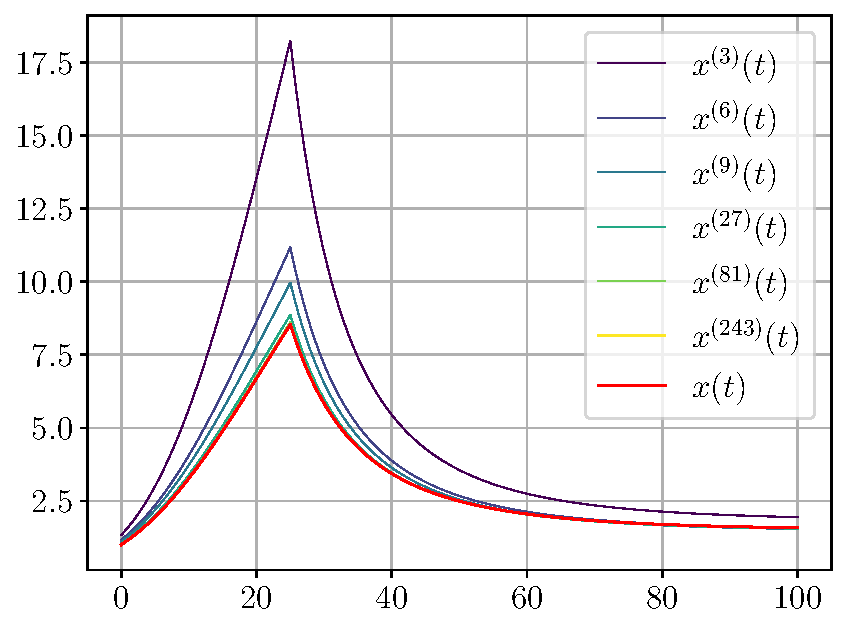
\includegraphics[scale=.7]{figs/theorem2.pdf}
        \caption{Sequence of solution trajectories.}
        \label{fig:th2}
    \end{figure}
    
\end{enumerate}


\subsection*{Problem \#2:}
\textit{
Consider a specific case of the CA system (\ref{eq:ca_sys}) from the paper. Assume that this specific system satisfies the conditions of Theorem \ref{th:3}.}
\begin{enumerate}[label=\alph*)]
    \item \textit{Discuss a constructive estimation for the trajectory $x(t)$ of (\ref{eq:ca_sys}) on a finite time interval $[0,t_f]$ using Theorem \ref{th:3}}.
    
    Consider the system
    \begin{equation}\label{eq:ex2}
        \begin{split}
            &\dot{x}(t)=0.5+e^{-t}u(t),\ \text{a.e. on } [0,1]\\
            &x(0)=0.
        \end{split}
    \end{equation}
    Let us prove that this system satisfies the conditions for Theorem \ref{th:3}. Let $C=[e^{-1},1]$, clearly $a(t,x)=0.5\in C$, $\forall t,x$. Moreover, $a(t,x)=e^{-t}\in C$, $\forall t,x$. Additionally, as $C$ is a closed and bounded interval in $\RR$, then it is compact and convex. Let $U=[-0.5,0.5]$, which satisfies that $0\in U$. Hence, the considered control system (\ref{eq:ex2}) satisfies all the conditions for Theorem \ref{th:3}.
    
    Therefore, the trajectory satisfies 
    \begin{equation}
        x(t)\in x_0+tC[1+\mathrm{diam}(U)]\implies x(t)\in \left[2e^{-2}t, 2t\right]
    \end{equation}
    
    \item \textit{Apply this trajectory estimation from Theorem \ref{th:3} to a simple example of the general system (\ref{th:3}).}
    
    In order to verify this estimation, we will consider three different admissible control functions in $U$: i) $u_1(t)=0.25,\ \forall t\in[0,1]$, ii) $u_2(t)=-0.25,\ \forall t\in[0,1]$ and iii) $u_3(t)=0.5\sin(4\pi t),\ \forall t\in[0,1]$. In Figure \ref{fig:th3}, the simulations of system (\ref{eq:ex2}) are presented for the three controllers; again, the expected result is obtained: the trajectories are inside the estimation for controllers in $U$.
    
    \begin{figure}[H]
        \centering
        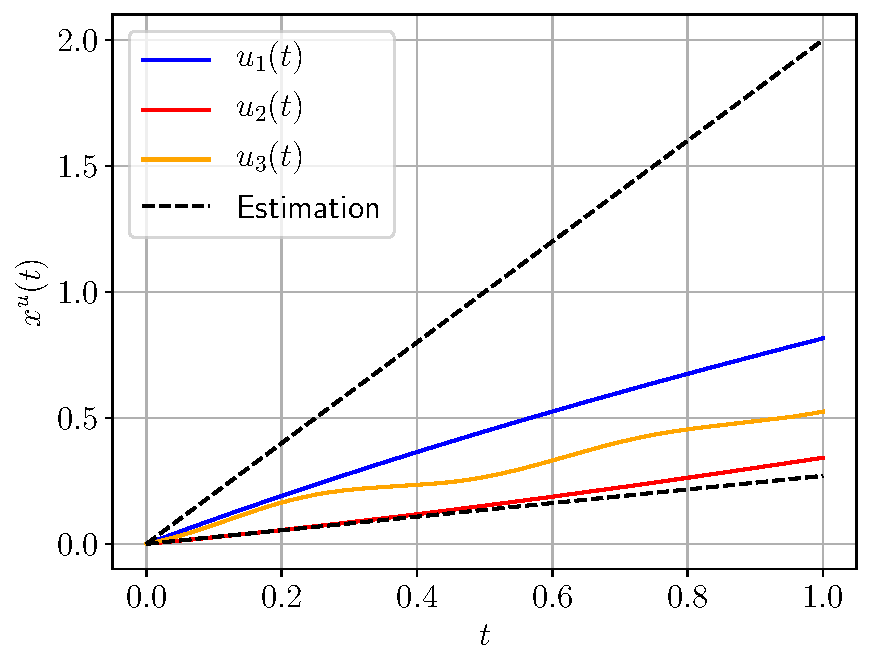
\includegraphics[scale=.7]{figs/theorem3.pdf}
        \caption{Simulation for three controllers in $U$.}
        \label{fig:th3}
    \end{figure}
    
\end{enumerate}


\subsection*{Problem \#3:}
\textit{
Consider the abstract Theorem \ref{th:1} from the paper application to the main dynamic system (\ref{eq:ca_sys}). Moreover, consider the proof of this Theorem \ref{th:1}.
\begin{enumerate}[label=\alph*)]
    \item Determine the concrete functional spaces $\X$, $\X^*$ (presented in the proof of Theorem \ref{th:1}) in the case of the dynamic system (\ref{eq:ca_sys}) that satisfies the conditions of Theorem \ref{th:2}.
    \item Determine the linear functional $\mathfrak{L}$ from the proof of Theorem \ref{th:1} in the framework of system (\ref{eq:ca_sys}) from Theorem \ref{th:2}0.
\end{enumerate}
}

The following answer for Problem \#3 is the result of a discussion with prof. Vadim, when we asked him about this exercise.

First, we may consider that both $x(\cdot)$ and $\dot{x}(\cdot)$ live in the same space $\X$, though $\dot{x}(\cdot)$ lives in manifold within $\X$ (tangent space). Accordingly to the theory of differential equations, and based on Carathéodory's existence theorem, the solution to (\ref{eq:ca_sys}) is a trajectory, which is an absolutely continuous function. Hence, we shall consider $\X\equiv AC(0,t_f)$. It can be proved that $AC(0,t_f)$ is Banach space with the norm
\[
\norm{f(\cdot)}_{AC(0,t_f)} = |f(0)|+\int_0^{t_f}\left|f'(t)\right|dt
\]
and it is well known that the corresponding dual to the space of absolutely continuous functions is the space of Radon measures. One main property of a Radon measure $\nu$ is that the integral
\[
\mathfrak{L} = \int \phi d\mu
\]
defines a positive linear functional in the space of absolutely continuous functions $\phi$. Hence, we define $\X^*$ as the space of Radon measures. It can be proved that $\X^*$ is a measure space (consequence of Radon-Nikodym's theorem). And the linear functionals $\mathfrak{L}\in\X^*$ are integrals in the space $\X$. For futher reading on these topics, refer for example to \cite{aliprantis1998principles} and \cite{bourbaki2003integration}.

\bibliographystyle{plain}
\bibliography{references}


\end{document}